\documentclass[paper=a4, fontsize=11pt]{scrartcl} 

\usepackage[T1]{fontenc} 
\usepackage[english]{babel}
\usepackage{amsmath,amsfonts,amsthm}

\usepackage{lipsum}

\usepackage{graphicx}
\usepackage{float}
  \floatplacement{figure}{H}
  \floatplacement{table}{H}
  
\usepackage{sectsty} 
\allsectionsfont{\centering \normalfont\scshape} 

\usepackage{fancyhdr} % Custom headers and footers
\pagestyle{fancyplain} % Makes all pages in the document conform to the custom headers and footers
\fancyhead{} % No page header - if you want one, create it in the same way as the footers below
\fancyfoot[L]{} % Empty left footer
\fancyfoot[C]{} % Empty center footer
\fancyfoot[R]{\thepage} % Page numbering for right footer
\renewcommand{\headrulewidth}{0pt} % Remove header underlines
\renewcommand{\footrulewidth}{0pt} % Remove footer underlines
\setlength{\headheight}{13.6pt} % Customize the height of the header

\numberwithin{equation}{section} % Number equations within sections (i.e. 1.1, 1.2, 2.1, 2.2 instead of 1, 2, 3, 4)
\numberwithin{figure}{section} % Number figures within sections (i.e. 1.1, 1.2, 2.1, 2.2 instead of 1, 2, 3, 4)
\numberwithin{table}{section} % Number tables within sections (i.e. 1.1, 1.2, 2.1, 2.2 instead of 1, 2, 3, 4)

\setlength\parindent{0pt} % Removes all indentation from paragraphs - comment this line for an assignment with lots of text

%----------------------------------------------------------------------------------------
%	TITLE SECTION
%----------------------------------------------------------------------------------------

\newcommand{\horrule}[1]{\rule{\linewidth}{#1}} % Create horizontal rule command with 1 argument of height

\title{	
\normalfont \normalsize 
\textsc{Computational Science - ITB} \\ [25pt] % Your university, school and/or department name(s)
\horrule{0.5pt} \\[0.4cm] % Thin top horizontal rule
%\huge  Summary - Euler Method\\ % The assignment title
%\horrule{2pt} \\[0.5cm] % Thick bottom horizontal rule
}

\author{\small{Ridlo W. Wibowo || 20912009}} % Your name

\date{\normalsize\today} % Today's date or a custom date

\begin{document}

\maketitle % Print the title

\large \textbf{Soal 1.}
Selesaikan SPL di bawah ini menggunakan metode iteratif:
\begin{eqnarray}
	4x_{1} - x_{2} \hspace{0.8cm}  - x_{4} \hspace{0.8cm} \hspace{0.8cm} &=& 0 \nonumber \\
	- x_{1} + 4x_{2} - x_{3} \hspace{0.8cm} - x_{5} \hspace{0.8cm} &=& 5 \nonumber \\
	\hspace{0.8cm} - x_{2} + 4x_{3}  \hspace{0.8cm} \hspace{0.8cm} - x_{6} &=& 0 \nonumber \\
	- x_{1} \hspace{0.8cm} \hspace{0.8cm} + 4x_{4} - x_{5} \hspace{0.8cm} &=& 6 \nonumber \\
	\hspace{0.8cm} - x_{2} \hspace{0.8cm} - x_{4} + 4x_{5} - x_{6} &=& -2 \nonumber \\
	\hspace{0.8cm} \hspace{0.8cm} - x_{3} \hspace{0.8cm} - x_{5} + 4x_{6} &=& 6 \nonumber \\
\end{eqnarray}
SPL di atas dapat diubah dalam bentuk matrix:\\
\begin{equation}
 Ax = b
\end{equation}
\[
 \begin{bmatrix}
  4 & -1 & 0 & -1 & 0 & 0 \\
  -1 & 4 & -1 & 0 & -1 & 0 \\
  0 & -1 & 4 & 0 & 0 & -1 \\
  -1 & 0 & 0 & 4 & -1 & 0 \\
 0 & -1 & 0 & -1 & 4 & -1 \\
  0 & 0 & -1 & 0 & -1 & 4 
 \end{bmatrix}
 \begin{bmatrix}
  x_{1} \\
  x_{2} \\
  x_{3} \\
  x_{4} \\
  x_{5} \\
  x_{6} 
 \end{bmatrix}
=
 \begin{bmatrix}
  0 \\
  5 \\
  0 \\
  6 \\
  -2 \\
  6 
 \end{bmatrix}
\]
terlihat bahwa matriks $A$ merupakan matriks yang dominan diagonal kuat, sehingga metode iteratif akan selalu mendapatkan solusi untuk semua tebakan awal $x^{(0)}$.\\
Kita akan menggunakan metode iteratif dalam menyelesaikan SPL ini, yaitu metode Jacobi dan Gauss-Seidel, dengan tebakan awal $x^{(0)} = [0, 0, 0, 0, 0, 0]^{T}$ dan $epsilon = 1.0\times 10^{-5}$\\

\newpage
\textbf{\large Iterasi Jacobi}\\
\textit{\textbf{Skema iterasi Jacobi}}:\\
\begin{equation}
x_{i}^{(k)} = \frac{1}{a_{ii}}\left(b_{i} -\sum_{{j=1}, {j\neq i}}^{n}a_{ij}x_{j}^{(k-1)} \right)
\end{equation}

\textit{\textbf{Algoritma iterasi Jacobi}}:\\
\textit{Input}\\
Vektor solusi tebakan awal $x^{(0)}$, toleransi $eps$ dan iterasi maksimum $Nmax$.\\

\textit{Output}\\
Vektor solusi hingga tercapai toleransi dan jumlah iterasi.\\

\textit{Langkah-langkah}
\begin{enumerate}
\item Set $xi_{i} = xo_{i}$ (tebakan awal) dan k = 0
\item Lakukan untuk $xf_{i} = \frac{1}{a_{ii}}\left(b_{i} \sum_{{j=1}, {j\neq i}}^{n}a_{ij}xi_{j} \right)$
\item Hitung Infinity Norm dari $(xf_{i} - xi_{i})$ dan ($xi_{i}$)
\item Hitung epsilon = Infinity Norm($xf_{i} - xi_{i}$)/Infinity Norm($xi_{i}$)
\item k ++
\item Swap $xi_{i} = xf_{i}$
\item Cek apakah $epsilon < toleransi$ dan $k < Nmax$, jika iya, kembali ke langkah 2, jika tidak hentikan program.
\end{enumerate}

\textit{\textbf{Program}}:
\begin{small}
\begin{verbatim}
#include <iostream>
#include <stdio.h>
#include <math.h>
using namespace std;
int main(){    
    int i, j, k=0, Nmax=100000;
    int n=6;
    double A['n']['n']={{4., -1., 0., -1., 0., 0.},
                        {-1., 4., -1., 0., -1., 0.},
                        {0., -1., 4., 0., 0., -1.},
                        {-1., 0., 0., 4., -1., 0.},
                        {0., -1., 0., -1., 4., -1.},
                        {0., 0., -1., 0., -1., 4.}};
    double b['n']={0., 5., 0., 6., -2., 6.};
    double xi['n']={0., 0., 0., 0., 0., 0.};
    double ep=0.00001;
    double xf['n'], eps, sum, vnorm_f['n'], norm_i, norm_f;

    cout << "### Program Jacobi untuk menyelesaikan SPL Ax=b ###\n";
    
    cout << "Matriks A : \n";
    for (i=0; i<n; i++){
        for (j=0; j<n; j++){ 
           cout << A[i][j] << "\t";}
        cout << "\n";}
    cout << "Vektor b : \n";
    for (i=0;i<n;i++){\newpage
        cout << b[i] << "\t";}
    cout << endl;
    cout << "Tebakan awal x(k=0): \n";
    for (i=0;i<n;i++){
        cout << xi[i] << " ";}
    cout << endl; 
    cout << "epsilon : " << ep << endl;
    // Jacobi method 
    cout << "Nilai barisan solusi x(k) dan epsilon : \n";
    do {
        for (i=0;i<n;i++){
            sum = 0.;
            for (j=0;j<n;j++){
                if (j != i){
                sum = sum - A[i][j]*xi[j];}}
            xf[i] =  (b[i] + sum)/A[i][i];}
        
        // menghitung epsilon dari Infinity Norm
        for (i=0;i<n;i++){
            vnorm_f[i] = xf[i] - xi[i];}
        norm_f = fabs(vnorm_f[0]);
        norm_i = fabs(xf[0]);
        for (i=1;i<n;i++){
            if (fabs(vnorm_f[i]) > norm_f){norm_f = fabs(vnorm_f[i]);}
            if (fabs(xf[i]) > norm_i){norm_i = fabs(xf[i]);}
        }
        eps = norm_f/norm_i;
        k ++;

        for (i=0;i<n;i++){
            xi[i] = xf[i]; // tukar x(k) dengan x(k+1)
            printf("%7.4f ", xf[i]);}
        cout << "\t" << eps;
        cout << endl;

    } while (eps > ep && k < Nmax);
    cout << "Jumlah iterasi : " << k << endl;
    return 0;}
\end{verbatim}
\end{small}

\textit{\textbf{Hasil}}:
\begin{small}
\begin{verbatim}
### Program Jacobi untuk menyelesaikan SPL Ax=b ###
Matriks A : 
4	-1	0	-1	0	0	
-1	4	-1	0	-1	0	
0	-1	4	0	0	-1	
-1	0	0	4	-1	0	
0	-1	0	-1	4	-1	
0	0	-1	0	-1	4	
Vektor b : 
0	5	0	6	-2	6	
Tebakan awal x(k=0): 
0 0 0 0 0 0 
epsilon : 1e-05
Nilai barisan solusi x(k) dan epsilon : 
 0.0000  1.2500  0.0000  1.5000 -0.5000  1.5000 	1
 0.6875  1.1250  0.6875  1.3750  0.5625  1.3750 	0.772727
 0.6250  1.7344  0.6250  1.8125  0.4688  1.8125 	0.336207
 0.8867  1.6797  0.8867  1.7734  0.8398  1.7734 	0.209251
 0.8633  1.9033  0.8633  1.9316  0.8066  1.9316 	0.115774
 0.9587  1.8833  0.9587  1.9175  0.9417  1.9175 	0.07041
 0.9502  1.9648  0.9502  1.9751  0.9296  1.9751 	0.0412546
 0.9850  1.9575  0.9850  1.9699  0.9787  1.9699 	0.0249648
 0.9819  1.9872  0.9819  1.9909  0.9743  1.9909 	0.0149087
 0.9945  1.9845  0.9945  1.9890  0.9923  1.9890 	0.0090067
 0.9934  1.9953  0.9934  1.9967  0.9907  1.9967 	0.00541521
 0.9980  1.9944  0.9980  1.9960  0.9972  1.9960 	0.00326949
 0.9976  1.9983  0.9976  1.9988  0.9966  1.9988 	0.00197056
 0.9993  1.9979  0.9993  1.9985  0.9990  1.9985 	0.00118949
 0.9991  1.9994  0.9991  1.9996  0.9988  1.9996 	0.000717555
 0.9997  1.9993  0.9997  1.9995  0.9996  1.9995 	0.000433102
 0.9997  1.9998  0.9997  1.9998  0.9995  1.9998 	0.000261352
 0.9999  1.9997  0.9999  1.9998  0.9999  1.9998 	0.000157742
 0.9999  1.9999  0.9999  1.9999  0.9998  1.9999 	9.51996e-05
 1.0000  1.9999  1.0000  1.9999  1.0000  1.9999 	5.74584e-05
 1.0000  2.0000  1.0000  2.0000  0.9999  2.0000 	3.46784e-05
 1.0000  2.0000  1.0000  2.0000  1.0000  2.0000 	2.09303e-05
 1.0000  2.0000  1.0000  2.0000  1.0000  2.0000 	1.26324e-05
 1.0000  2.0000  1.0000  2.0000  1.0000  2.0000 	7.62435e-06
Jumlah iterasi : 24
\end{verbatim}
\end{small}

\vspace{1cm}
\textbf{\large Iterasi Gauss-Seidel}\\
\textit{\textbf{Skema iterasi Gauss-Seidel}}:\\
\begin{equation}
x_{i}^{(k)} = \frac{1}{a_{ii}}\left(b_{i} -\sum_{j=1}^{i-1}a_{ij}x_{j}^{(k)} -\sum_{j=i+1}^{n}a_{ij}x_{j}^{(k-1)}\right)
\end{equation}

\textit{\textbf{Algoritma iterasi Gauss-Seidel}}:\\
\textit{Input}\\
Vektor solusi tebakan awal $x^{(0)}$, toleransi $eps$ dan iterasi maksimum $Nmax$.\\

\textit{Output}\\
Vektor solusi hingga tercapai toleransi dan jumlah iterasi.\\

\textit{Langkah-langkah}
\begin{enumerate}
\item Set $xi_{i} = xo_{i}$ (tebakan awal) dan k = 0
\item Lakukan untuk $xf_{i} = \frac{1}{a_{ii}}\left(b_{i} -\sum_{j=1}^{i-1}a_{ij}xf_{j} -\sum_{j=i+1}^{n}a_{ij}xi_{j}\right)$
\item Hitung Infinity Norm dari $(xf_{i} - xi_{i})$ dan ($xi_{i}$)
\item Hitung epsilon = Infinity Norm($xf_{i} - xi_{i}$)/Infinity Norm($xi_{i}$)
\item k ++
\item Swap $xi_{i} = xf_{i}$
\item Cek apakah $epsilon < toleransi$ dan $k < Nmax$, jika iya, kembali ke langkah 2, jika tidak hentikan program.
\end{enumerate}

\textit{\textbf{Program}}:
\begin{small}
\begin{verbatim}
#include <iostream>
#include <stdio.h>
#include <math.h>
using namespace std;
int main(){    
    int i, j, k=0, Nmax=100000;
    int n=6;
    double A['n']['n']={{4., -1., 0., -1., 0., 0.},
                        {-1., 4., -1., 0., -1., 0.},
                        {0., -1., 4., 0., 0., -1.},
                        {-1., 0., 0., 4., -1., 0.},
                        {0., -1., 0., -1., 4., -1.},
                        {0., 0., -1., 0., -1., 4.}};
    double b['n']={0., 5., 0., 6., -2., 6.};
    double xi['n']={0., 0., 0., 0., 0., 0.};
    double ep=0.00001;
    double omega=1.1;
    double xf['n'], eps, sum_a, sum_b, vnorm_f['n'], norm_i, norm_f;
    cout << "### Program Gauss-Seidel untuk menyelesaikan SPL Ax=b ###\n";    
    cout << "Matriks A : \n";
    for (i=0; i<n; i++){
        for (j=0; j<n; j++){ 
           cout << A[i][j] << "\t";}
        cout << "\n";}
    cout << "Vektor b : \n";
    for (i=0;i<n;i++){
        cout << b[i] << "\t";}
    cout << endl;
    cout << "Tebakan awal x(k=0): \n";
    for (i=0;i<n;i++){
        cout << xi[i] << " ";}
    cout << endl; 
    cout << "epsilon : " << ep << endl;
    // Gauss-Seidel method 
    cout << "Nilai barisan solusi x(k) dan epsilon : \n";
    do { 		// iterasi
        for (i=0;i<n;i++){
            sum_a = 0.;
            sum_b = 0.;
                for (j=0;j<=i-1;j++){
                    if (j != i){
                    sum_a = sum_a - A[i][j]*xf[j];}}
                for (j=i+1;j<=n;j++){
                    if (j != i){
                    sum_b = sum_b - A[i][j]*xi[j];}}
            xf[i] = (b[i] + sum_a + sum_b)/A[i][i];}
        
        // menghitung epsilon dari Infinity Norm
        for (i=0;i<n;i++){
            vnorm_f[i] = xf[i] - xi[i];}
        norm_f = fabs(vnorm_f[0]);
        norm_i = fabs(xf[0]);
        for (i=1;i<n;i++){
            if (fabs(vnorm_f[i]) > norm_f){norm_f = fabs(vnorm_f[i]);}
            if (fabs(xf[i]) > norm_i){norm_i = fabs(xf[i]);}
        }
        eps = norm_f/norm_i;
        k ++;      
        for (i=0;i<n;i++){
            xi[i] = xf[i]; // tukar x(k) dengan x(k+1)
            printf("%7.4f ", xf[i]);}
        cout << "\t" << eps;
        cout << endl;

    } while (eps > ep && k < Nmax); // penghenti iterasi
    cout << "Jumlah iterasi : " << k << endl;
    return 0;
}
\end{verbatim}
\end{small}

\textit{\textbf{Hasil}}:
\begin{small}
\begin{verbatim}
### Program Gauss-Seidel untuk menyelesaikan SPL Ax=b ###
Matriks A : 
4	-1	0	-1	0	0	
-1	4	-1	0	-1	0	
0	-1	4	0	0	-1	
-1	0	0	4	-1	0	
0	-1	0	-1	4	-1	
0	0	-1	0	-1	4	
Vektor b : 
0	5	0	6	-2	6	
Tebakan awal x(k=0): 
0 0 0 0 0 0 
epsilon : 1e-05
Nilai barisan solusi x(k) dan epsilon : 
 0.0000  1.2500  0.3125  1.5000  0.1875  1.6250 	1
 0.6875  1.5469  0.7930  1.7188  0.7227  1.8789 	0.365904
 0.8164  1.8330  0.9280  1.8848  0.8992  1.9568 	0.146226
 0.9294  1.9391  0.9740  1.9572  0.9633  1.9843 	0.0569653
 0.9741  1.9778  0.9905  1.9843  0.9866  1.9943 	0.0223799
 0.9905  1.9919  0.9966  1.9943  0.9951  1.9979 	0.00824212
 0.9966  1.9971  0.9987  1.9979  0.9982  1.9992 	0.00300691
 0.9987  1.9989  0.9995  1.9992  0.9994  1.9997 	0.00109549
 0.9995  1.9996  0.9998  1.9997  0.9998  1.9999 	0.000399051
 0.9998  1.9999  0.9999  1.9999  0.9999  2.0000 	0.000145362
 0.9999  1.9999  1.0000  2.0000  1.0000  2.0000 	5.29515e-05
 1.0000  2.0000  1.0000  2.0000  1.0000  2.0000 	1.92889e-05
 1.0000  2.0000  1.0000  2.0000  1.0000  2.0000 	7.02649e-06
Jumlah iterasi : 13
\end{verbatim}
\end{small}

\vspace{1cm}
Kita dapat melakukan sedikit perubahan pada metode Gauss-Seidel ini agar lebih cepat konvergen. Banyak kasus yang terjadi pada metode iteratif yakni perubahan $x_{i}$ selalu menuju ke arah yang sama (tidak berosilasi). Sehingga \textit{over-correcting} (\textit{over-relaxing}) untuk $x_{i}$ dengan nilai yang tepat dapat mempercepat kekonvergenan. Hal ini dapat diilustrasikan seperti gambar di bawah ini.

\begin{figure}
	\centering
	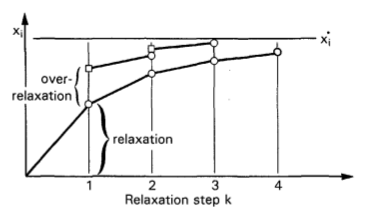
\includegraphics[width=0.5\textwidth]
		{sor.png}
	\caption{Over-relaxation.}
	\label{fig:sor}
\end{figure}

Dengan memasukkan faktor over-ralaksasi $\omega $ (biasanya $1.0<\omega<2.0$) maka kita peroleh metode yang kemudian biasa disebut sebagai metode \textit{Successive Over-Relaxation} (SOR).\\
Skema SOR :
\begin{equation}
x_{i}^{(k)} = (1 - \omega)x_{i}^{(k)} + \frac{\omega}{a_{ii}}\left(b_{i} -\sum_{j=1}^{i-1}a_{ij}x_{j}^{(k)} -\sum_{j=i+1}^{n}a_{ij}x_{j}^{(k-1)}\right)
\end{equation}

dengan menggunakan skema di atas, kita dapat melakukan sedikit perubahan pada program Gauss-Seidel di atas. Untuk kasus yang sama dengan $\omega = 1.1$ diperoleh hasil iterasi:

\begin{small}
\begin{verbatim}
### Program Gauss-Seidel + Successive Over-Relaxation ###
Tebakan awal x(k=0): 
0 0 0 0 0 0 
epsilon   : 1e-05
omega SOR : 1.1
Nilai barisan solusi x(k) dan epsilon : 
 0.0000  1.3750  0.3781  1.6500  0.2819  1.8315 	1
 0.8319  1.6478  0.9190  1.7913  0.8712  1.9592 	0.424609
 0.8626  1.9397  0.9803  1.9477  0.9707  1.9906 	0.146671
 0.9828  1.9878  0.9960  1.9924  0.9949  1.9985 	0.0601595
 0.9963  1.9977  0.9993  1.9983  0.9990  1.9997 	0.00675739
 0.9993  1.9996  0.9999  1.9997  0.9998  1.9999 	0.00149757
 0.9999  1.9999  1.0000  1.9999  1.0000  2.0000 	0.000293119
 1.0000  2.0000  1.0000  2.0000  1.0000  2.0000 	5.2646e-05
 1.0000  2.0000  1.0000  2.0000  1.0000  2.0000 	9.94652e-06
Jumlah iterasi : 9
\end{verbatim}
\end{small}

\textbf{Analisis hasil dan kesimpulan}\\
Solusi eksak untuk SPL di atas adalah $x_{i} = [1, 2, 1, 2, 1, 2]^{T}$ dan dari program di atas terlihat bahwa:
\begin{enumerate}
\item Metode Gauss-Seidel lebih cepat konvergen dibandingkan dengan metode Jacobi. Metode Jacobi membutuhkan 24 kali iterasi sedangkan Gauss-Seidel hanya membutuhkan 13 kali iterasi, dengan toleransi yang sama yaitu $1.0\times 10^{-5}$.
\item Sedikit penambahan pada metode Gauss-Seidel kita peroleh skema \textit{Successive Over-Relaxation} (SOR), yang apabila kita memasukan $\omega $ yang tepat maka akan mempercepat kekonvergenan metode iterasi (9 kali iterasi dengan nilai $\omega = 1.1$ untuk nilai toleransi yang sama).
\end{enumerate}

\newpage
\large \textbf{Soal 2.}
Terdapat Sistem Persamaan Linier (SPL) sebagai berikut:
\begin{eqnarray}
	2x_{1} -  x_{2} +  x_{3} &=& -1 \nonumber \\
	2x_{1} + 2x_{2} + 2x_{3} &=&  4 \nonumber \\
	-x_{1} -  x_{2} + 2x_{3} &=& -5 \nonumber \\
\end{eqnarray}
yang mempunyai solusi eksak $x_{i} = [1, 2, -1]^T$\\
\begin{enumerate}
\item Tunjukkan bahwa $\rho(Tj) = \frac{\sqrt{5}}{2} > 1$.
\item Tunjukkan bahwa metode iterasi Jacobi dengan hampiran awal $x_{i}^{(0)} = 0$ akan gagal menghasilkan hampiran yang baik setelah 25 iterasi.
\item Tunjukkan bahwa $\rho(Tg) = \frac{1}{2}$.
\item Pergunakan iterasi Gauss-Seidel dengan hampiran awal $x_{i}^{(0)} = 0$ untuk mengjampiri solusi SPL dengan toleransi $10^{-5}$ dalam norm tak hingga ($L_{\infty}$).
\end{enumerate}
\textbf{Jawab}:\\
SPL dalam bentuk matriks $Ax = b$ :\\
\[
 \begin{bmatrix}
  2 & -1 & 1 \\
  2 &  2 & 2 \\
 -1 & -1 & 2
 \end{bmatrix}
 \begin{bmatrix}
  x_{1} \\
  x_{2} \\
  x_{3} 
 \end{bmatrix}
=
 \begin{bmatrix}
  -1 \\
  4 \\
  -5 
 \end{bmatrix}
\]

1. Tunjukkan $\rho(Tj) = \frac{\sqrt{5}}{2} > 1$\\

$Tj = D^{-1}(L + U)$, dengan\\

\[ 
D = 
\begin{bmatrix}
  2 & 0 & 0 \\
  0 & 2 & 0 \\
  0 & 0 & 2
 \end{bmatrix}
,
L = 
\begin{bmatrix}
  0 & 0 & 0 \\
 -2 & 0 & 0 \\
  1 & 1 & 0
 \end{bmatrix}
, 
U = 
\begin{bmatrix}
  0 & 1 & -1 \\
  0 & 0 & -2 \\
  0 & 0 &  0
 \end{bmatrix}
\]
sehingga diperoleh
\[
D^{-1} =
\begin{bmatrix}
  \frac{1}{2} & 0 & 0 \\
  0 & \frac{1}{2} & 0 \\
  0 & 0 & \frac{1}{2}
 \end{bmatrix}
\]
\[
Tj = D^{-1}(L + U) = 
\begin{bmatrix}
  \frac{1}{2} & 0 & 0 \\
  0 & \frac{1}{2} & 0 \\
  0 & 0 & \frac{1}{2}
\end{bmatrix}
\left(
\begin{bmatrix}
  0 & 0 & 0 \\
 -2 & 0 & 0 \\
  1 & 1 & 0
 \end{bmatrix}
+
\begin{bmatrix}
  0 & 1 & -1 \\
  0 & 0 & -2 \\
  0 & 0 &  0
 \end{bmatrix}
\right)
\]
\[
Tj = 
\begin{bmatrix}
  0 & \frac{1}{2} & -\frac{1}{2} \\
  -1 & 0 & -1 \\
  \frac{1}{2} & \frac{1}{2} & 0
\end{bmatrix}
\]
\[
det(Tj - \lambda I) =
\left| 
\begin{array}{ccc}
  -\lambda & \frac{1}{2} & -\frac{1}{2} \\
  -1 & -\lambda & -1 \\
  \frac{1}{2} & \frac{1}{2} & -\lambda 
\end{array} 
\right|
= -\lambda^{3} - \frac{5}{4}\lambda = -\lambda (\lambda^{2} + \frac{5}{4})
\]
di peroleh: $\lambda_{1} = 0$, $\lambda_{2} = -\sqrt{\frac{5}{4}}$, $\lambda_{3} = \sqrt{\frac{5}{4}}$\\
maka $\rho(Tj) = maks\lbrace \left| 0 \right|, \left| -\sqrt{\frac{5}{4}} \right|, \left| \sqrt{\frac{5}{4}} \right| \rbrace = \sqrt{\frac{5}{4}} > 1 $ (terbukti).\\


2. Dengan menggunakan program pada soal sebelumnya untuk kasus di atas, diperoleh output hingga iterasi ke 25 seperti di bawah ini (tidak konvergen walaupun jumlah iterasi ditambah).
\begin{small}
\begin{verbatim}
### Program Jacobi untuk menyelesaikan SPL Ax=b ###
Matriks A : 
2	-1	1	
2	2	2	
-1	-1	2	
Vektor b : 
-1	4	-5	
Tebakan awal x(k=0): 
0 0 0 
epsilon : 1e-05
Nilai barisan solusi x(k) dan epsilon : 
-0.5000  2.0000 -2.5000 	1
 1.7500  5.0000 -1.7500 	0.6
 2.8750  2.0000  0.8750 	1.04348
 0.0625 -1.7500 -0.0625 	2.14286
-1.3438  2.0000 -3.3438 	1.1215
 2.1719  6.6875 -2.1719 	0.700935
 3.9297  2.0000  1.9297 	1.19284
-0.4648 -3.8594  0.4648 	1.51822
-2.6621  2.0000 -4.6621 	1.25681
 2.8311  9.3242 -2.8311 	0.785505
 5.5776  2.0000  3.5776 	1.31314
-1.2888 -7.1553  1.2888 	1.27951
-4.7220  2.0000 -6.7220 	1.36198
 3.8610 13.4441 -3.8610 	0.851236
 8.1526  2.0000  6.1526 	1.40374
-2.5763 -12.3051  2.5763 	1.16253
-7.9407  2.0000 -9.9407 	1.43905
 5.4703 19.8814 -5.4703 	0.899403
12.1759  2.0000 10.1759 	1.46859
-4.5879 -20.3517  4.5879 	1.09827
-12.9698  2.0000 -14.9698 	1.49312
 7.9849 29.9397 -7.9849 	0.933199
18.4623  2.0000 16.4623 	1.51334
-7.7311 -32.9246  7.7311 	1.06074
-20.8279  2.0000 -22.8279 	1.52991
Jumlah iterasi : 25
\end{verbatim}
\end{small}

3. Tunjukkan $\rho(Tg) = \frac{1}{2} < 1$ (akan konvergen)\\
$Tg = (D-L)^{-1}U$, dengan\\
\[ 
D = 
\begin{bmatrix}
  2 & 0 & 0 \\
  0 & 2 & 0 \\
  0 & 0 & 2
 \end{bmatrix}
,
L = 
\begin{bmatrix}
  0 & 0 & 0 \\
 -2 & 0 & 0 \\
  1 & 1 & 0
 \end{bmatrix}
, 
U = 
\begin{bmatrix}
  0 & 1 & -1 \\
  0 & 0 & -2 \\
  0 & 0 &  0
 \end{bmatrix}
\]
sehingga diperoleh
\[
D-L =
\begin{bmatrix}
  2 & 0 & 0 \\
  2 & 2 & 0 \\
  -1 & -1 & 2
 \end{bmatrix}
,
(D-L)^{-1} =
\begin{bmatrix}
  \frac{1}{2} & 0 & 0 \\
  -\frac{1}{2} & \frac{1}{2} & 0 \\
  0 & \frac{1}{4} & \frac{1}{2}
 \end{bmatrix}
\]
\[
Tg = (D-L)^{-1}U = 
\begin{bmatrix}
  \frac{1}{2} & 0 & 0 \\
  -\frac{1}{2} & \frac{1}{2} & 0 \\
  0 & \frac{1}{4} & \frac{1}{2}
 \end{bmatrix}
\begin{bmatrix}
  0 & 1 & -1 \\
  0 & 0 & -2 \\
  0 & 0 &  0
 \end{bmatrix}
\]
\[
Tg = 
\begin{bmatrix}
  0 & \frac{1}{2} & -\frac{1}{2} \\
  0 & -\frac{1}{2} & -\frac{1}{2} \\
  0 & 0 & -\frac{1}{2}
\end{bmatrix}
\]
\[
det(Tg - \lambda I) =
\left| 
\begin{array}{ccc}
  -\lambda & \frac{1}{2} & -\frac{1}{2} \\
  0 & -\frac{1}{2}-\lambda & -\frac{1}{2} \\
  0 & 0 & -\frac{1}{2}-\lambda
\end{array} 
\right|
= -\lambda(\frac{1}{2} + \lambda)^{2} 
\]
di peroleh: $\lambda_{1} = 0$, $\lambda_{2} = -\frac{1}{2}$, $\lambda_{3} = \frac{1}{2}$\\
maka $\rho(Tg) = maks\lbrace \left| 0 \right|, \left| -\frac{1}{2} \right|, \left| \frac{1}{2} \right| \rbrace = \frac{1}{2} < 1 $ (terbukti).\\

4. Dengan menggunakan program Gauss-Seidel pada soal sebelumnya untuk nilai toleransi $10^{-5}$ menggunakan $l_{\infty}$ diperoleh hasil seperti di bawah ini.
\begin{small}
\begin{verbatim}
### Program Gauss-Seidel untuk menyelesaikan SPL Ax=b ###
Matriks A : 
2	-1	1	
2	2	2	
-1	-1	2	
Vektor b : 
-1	4	-5	
Tebakan awal x(k=0): 
0 0 0 
epsilon : 1e-05
Nilai barisan solusi x(k) dan epsilon : 
-0.5000  2.5000 -1.5000 	1
 1.5000  2.0000 -0.7500 	1
 0.8750  1.8750 -1.1250 	0.333333
 1.0000  2.1250 -0.9375 	0.117647
 1.0312  1.9062 -1.0312 	0.114754
 0.9688  2.0625 -0.9844 	0.0757576
 1.0234  1.9609 -1.0078 	0.0517928
 0.9844  2.0234 -0.9961 	0.030888
 1.0098  1.9863 -1.0020 	0.0186824
 0.9941  2.0078 -0.9990 	0.0107004
 1.0034  1.9956 -1.0005 	0.00611696
 0.9980  2.0024 -0.9998 	0.0034138
 1.0011  1.9987 -1.0001 	0.00189336
 0.9994  2.0007 -0.9999 	0.00103722
 1.0003  1.9996 -1.0000 	0.000564687
 0.9998  2.0002 -1.0000 	0.000305143
 1.0001  1.9999 -1.0000 	0.000164041
 0.9999  2.0001 -1.0000 	8.77354e-05
 1.0000  2.0000 -1.0000 	4.67308e-05
 1.0000  2.0000 -1.0000 	2.47953e-05
 1.0000  2.0000 -1.0000 	1.31131e-05
 1.0000  2.0000 -1.0000 	6.91412e-06
Jumlah iterasi : 22
\end{verbatim}
\end{small}
Hasil di atas menunjukkan bahwa dengan menggunakan iterasi gauss-seidel solusinya konvergen menuju solusi eksak untuk toleransi $10^{-5}$ setelah iterasi ke 22.\\

\vspace{1cm}
\large \textbf{Soal 3.}
Carilah akar-akar dari sistem persamaan nonlinier berikut ini menggunakan metode Newton.\\
\begin{eqnarray}
f_{1}(x_{1}, x_{2}) &=& 0.5\sin(x_{1}x_{2}) - 0.25\frac{x_{2}}{\pi} - 0.5x_{1}\\
f_{2}(x_{1}, x_{2}) &=& (1-\frac{0.25}{\pi})(exp(2x_{1} - e) + e\frac{x_{2}}{\pi} - 2ex_{1}
\end{eqnarray}

Jika kita gambar 2 fungsi di atas untuk $z=0$ dengan $ -1<x<3 $ dan $ -20<y<5 $ maka diperoleh kurva seperti berikut:

\begin{figure}
	\centering
	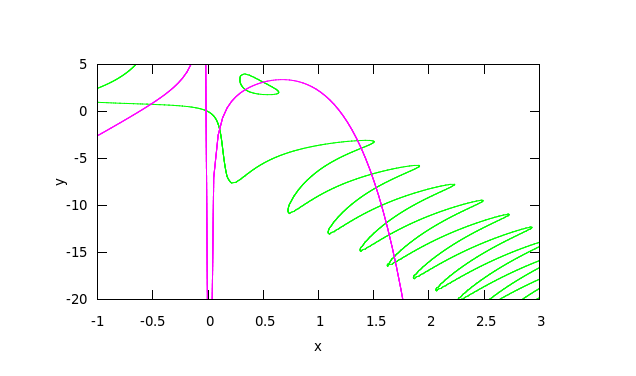
\includegraphics[width=1.0\textwidth]
		{plot3.png}
	\caption{$f_{1}(x_{1}, x_{2})$ dan $f_{2}(x_{1}, x_{2})$.}
	\label{fig:plot3}
\end{figure}

\end{document}














